\documentclass[10pt,a4paper]{article}

% Packages
\usepackage{fancyhdr}           % For header and footer
\usepackage{multicol}           % Allows multicols in tables
\usepackage{tabularx}           % Intelligent column widths
\usepackage{tabulary}           % Used in header and footer
\usepackage{hhline}             % Border under tables
\usepackage{graphicx}           % For images
\usepackage{xcolor}             % For hex colours
%\usepackage[utf8x]{inputenc}    % For unicode character support
\usepackage[T1]{fontenc}        % Without this we get weird character replacements
\usepackage{colortbl}           % For coloured tables
\usepackage{setspace}           % For line height
\usepackage{lastpage}           % Needed for total page number
\usepackage{seqsplit}           % Splits long words.
%\usepackage{opensans}          % Can't make this work so far. Shame. Would be lovely.
\usepackage[normalem]{ulem}     % For underlining links
% Most of the following are not required for the majority
% of cheat sheets but are needed for some symbol support.
\usepackage{amsmath}            % Symbols
\usepackage{MnSymbol}           % Symbols
\usepackage{wasysym}            % Symbols
%\usepackage[english,german,french,spanish,italian]{babel}              % Languages

% Document Info
\author{namorDev}
\pdfinfo{
  /Title (Conan Cheatsheet NoEng Kickoff 2022.pdf)
  /Creator (Noser Engineering AG)
  /Author (Roman Baertschi)
  /Subject (Conan Cheat Sheet)
}


\graphicspath{ {./images/} }

% Lengths and widths
\addtolength{\textwidth}{6cm}
\addtolength{\textheight}{-1cm}
\addtolength{\hoffset}{-3cm}
\addtolength{\voffset}{-2cm}
\setlength{\tabcolsep}{0.2cm} % Space between columns
\setlength{\headsep}{-12pt} % Reduce space between header and content
\setlength{\headheight}{85pt} % If less, LaTeX automatically increases it
\renewcommand{\footrulewidth}{0pt} % Remove footer line
\renewcommand{\headrulewidth}{0pt} % Remove header line
\renewcommand{\seqinsert}{\ifmmode\allowbreak\else\-\fi} % Hyphens in seqsplit
% This two commands together give roughly
% the right line height in the tables
\renewcommand{\arraystretch}{1.3}
\onehalfspacing

% Commands
\newcommand{\SetRowColor}[1]{\noalign{\gdef\RowColorName{#1}}\rowcolor{\RowColorName}} % Shortcut for row colour
\newcommand{\mymulticolumn}[3]{\multicolumn{#1}{>{\columncolor{\RowColorName}}#2}{#3}} % For coloured multi-cols
\newcolumntype{x}[1]{>{\raggedright}p{#1}} % New column types for ragged-right paragraph columns
\newcommand{\tn}{\tabularnewline} % Required as custom column type in use

% Font and Colours
\definecolor{HeadBackground}{HTML}{333333}
\definecolor{FootBackground}{HTML}{666666}
\definecolor{TextColor}{HTML}{333333}
\definecolor{DarkBackground}{HTML}{FA9400}
\definecolor{LightBackground}{HTML}{DFEBFF}
\renewcommand{\familydefault}{\sfdefault}
\color{TextColor}

% Header and Footer
\pagestyle{fancy}
\fancyhead{} % Set header to blank
\fancyfoot{} % Set footer to blank
\fancyhead[L]{
\noindent
\begin{multicols}{3}
% -
\columnbreak
\begin{tabulary}{11cm}{L}
    \vspace{-2pt}\large{\bf{\textcolor{DarkBackground}{\textrm{Conan - C/C++ Package Manager}}}}
\end{tabulary}
\end{multicols}}

\fancyfoot[L]{ \footnotesize
\noindent
\begin{multicols}{3}
\begin{tabulary}{5.8cm}{LL}
  \SetRowColor{FootBackground}
  \mymulticolumn{2}{p{5.377cm}}{\bf\textcolor{white}{Cheatsheet Template}}  \\
  \vspace{-2pt}emmajane \\
  \uline{cheatography.com/emmajane} \\
  \end{tabulary}
\vfill
\columnbreak
\begin{tabulary}{5.8cm}{L}
  \SetRowColor{FootBackground}
  \mymulticolumn{1}{p{5.377cm}}{\bf\textcolor{white}{Cheat Sheet creator}}  \\
   \vspace{-2pt} namorDev\\
   \uline{https://github.com/namorDev/Conan-\\
   	Cheatsheet} \\
\end{tabulary}
\vfill
\columnbreak
\begin{tabulary}{5.8cm}{L}
  \SetRowColor{FootBackground}
  \mymulticolumn{1}{p{5.377cm}}{\bf\textcolor{white}{Event}}  \\
  \SetRowColor{white}
  \vspace{-2pt} Noser Engineering AG \\
  Kickoff 2022
\end{tabulary}
\end{multicols}}




\begin{document}
\raggedright
\raggedcolumns

% Set font size to small. Switch to any value
% from this page to resize cheat sheet text:
% www.emerson.emory.edu/services/latex/latex_169.html
\footnotesize % Small font.



adfad


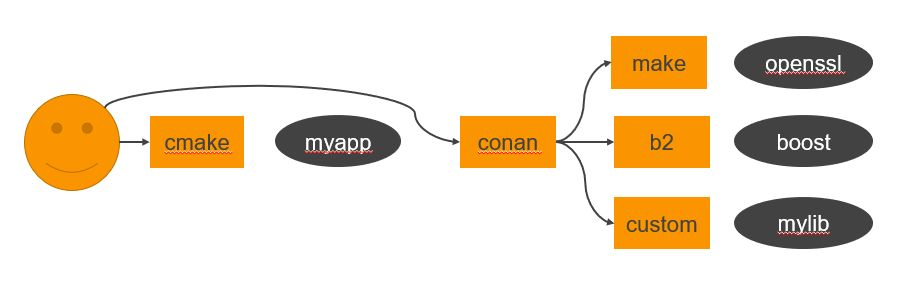
\includegraphics[scale=0.2]{BuildSystemAbstraction}


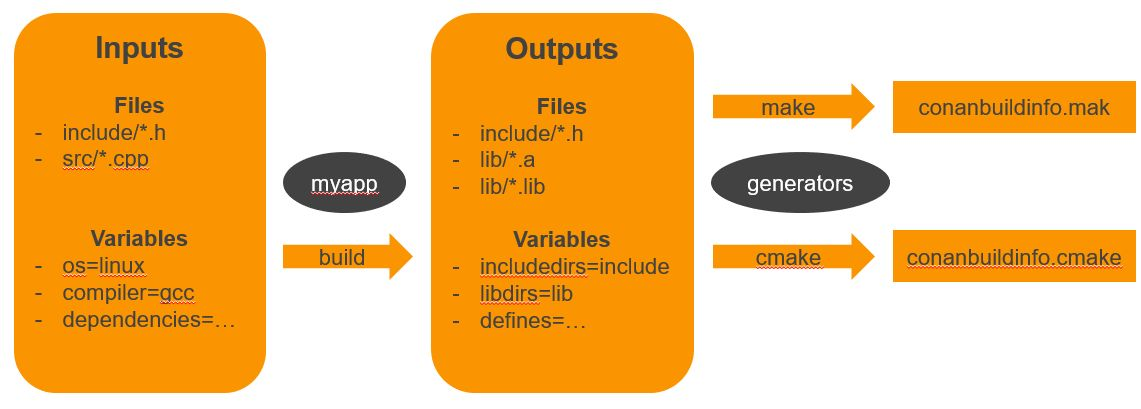
\includegraphics[scale=0.2]{Recipe_InOut}


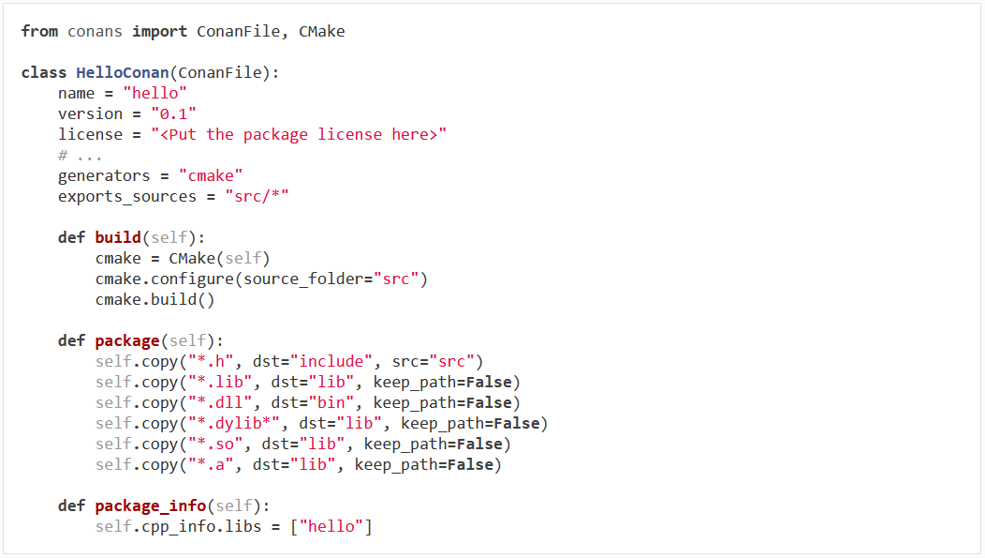
\includegraphics[scale=0.2]{Recipe}


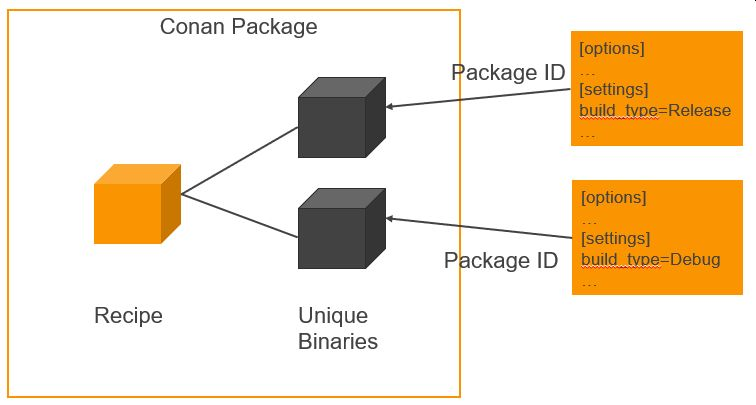
\includegraphics[scale=0.2]{BinaryManagement}


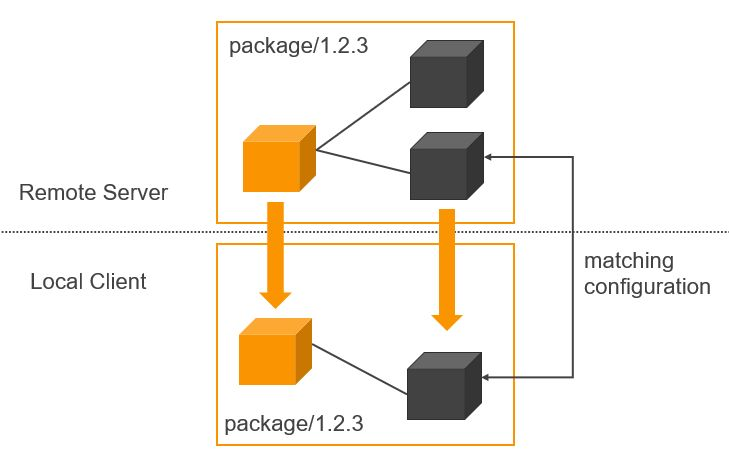
\includegraphics[scale=0.2]{BinaryManagement_RemoteLocal}





\pagebreak

\begin{multicols*}{3}


\vfill
\columnbreak
\begin{tabularx}{5.377cm}{X}
\SetRowColor{DarkBackground}
\mymulticolumn{1}{x{5.377cm}}{\bf\textcolor{white}{Consuming Packages}}  \tn

\SetRowColor{LightBackground}
\mymulticolumn{1}{x{5.377cm}}{{\bf{\$conan install <recipe\_reference>}} Install dependencies.} \tn 
% Row Count 1 (+ 1)
% Row 15
\SetRowColor{white}
\mymulticolumn{1}{x{5.377cm}}{{\bf{\$conan install . --build=missing}} Builds dependencies if no suitable binary found. "." specifies the location of the conanfile.} \tn 


\hhline{>{\arrayrulecolor{DarkBackground}}-}

\end{tabularx}
\par\addvspace{1.3em}

\begin{tabularx}{5.377cm}{X}
\SetRowColor{DarkBackground}
\mymulticolumn{1}{x{5.377cm}}{\bf\textcolor{white}{Creating Packages}}  \tn
% Row 0
\SetRowColor{LightBackground}
\mymulticolumn{1}{x{5.377cm}}{{\bf{\$conan create hello/0.1}} Creates a package and stores it to local cache} \tn 

% Row Count 8 (+ 2)
% Row 4
\SetRowColor{LightBackground}
\mymulticolumn{1}{x{5.377cm}}{{\bf{\$conan new <recipe\_reference>}} Creates a new recipe with boilerplate code.} \tn 


\SetRowColor{white}
\mymulticolumn{1}{x{5.377cm}}{{\bf{\$conan new hello}} Creates a new recipe from the hello template} \tn 
% Row Count 6 (+ 5)
% Row 2
\SetRowColor{LightBackground}
\mymulticolumn{1}{x{5.377cm}}{{\bf{\$conan build}} Builds a package. Invokes the build method} \tn 
% Row Count 7 (+ 1)
% Row 3
\SetRowColor{white}
\mymulticolumn{1}{x{5.377cm}}{{\bf{\$conan export}} Export recipe to local cache but does not build it} \tn 

\hhline{>{\arrayrulecolor{DarkBackground}}-}
\end{tabularx}
\par\addvspace{1.3em}

\begin{tabularx}{5.377cm}{X}
\SetRowColor{DarkBackground}
\mymulticolumn{1}{x{5.377cm}}{\bf\textcolor{white}{Inspecting Packages}}  \tn
% Row 0
\SetRowColor{LightBackground}
\mymulticolumn{1}{x{5.377cm}}{{\bf{\$conan search}} Lists all packages in local cache} \tn 

\SetRowColor{white}
\mymulticolumn{1}{x{5.377cm}}{{\bf{\$conan search <package\_reference>}} Shows info about package. No info, if no binaries existing} \tn 
% Row Count 2 (+ 1)
\hhline{>{\arrayrulecolor{DarkBackground}}-}
\SetRowColor{LightBackground}
\mymulticolumn{1}{x{5.377cm}}{{\bf{\$conan info}} Shows dependencies of a package.} \tn 
\hhline{>{\arrayrulecolor{DarkBackground}}-}
\end{tabularx}
\par\addvspace{1.3em}

\begin{tabularx}{5.377cm}{X}
	\SetRowColor{DarkBackground}
	\mymulticolumn{1}{x{5.377cm}}{\bf\textcolor{white}{Working with remotes}}  \tn
	% Row 0
	\SetRowColor{LightBackground}
	\mymulticolumn{1}{x{5.377cm}}{{\bf{\$conan upload}} Uploads a package to a remote} \tn 
	% Row Count 1 (+ 1)
	% Row 1
	\SetRowColor{white}
	\mymulticolumn{1}{x{5.377cm}}{{\bf{\$conan remote list}} shows remote repositories} \tn 
	% Row Count 2 (+ 1)
	% Row 2
	\SetRowColor{LightBackground}
	\mymulticolumn{1}{x{5.377cm}}{{\bf{conan center}} Default remote repo} \tn 
	
	\SetRowColor{white}
	\mymulticolumn{1}{x{5.377cm}}{{\bf{conan remote add <remote\_repo\_name> <url>}} Adds a remote repository} \tn 
	
	\SetRowColor{LightBackground}
    \mymulticolumn{1}{x{5.377cm}}{{\bf{conan search -r=<remote\_repo\_name>}} Searches for packages in a remote repo} \tn 

	\SetRowColor{white}
	\mymulticolumn{1}{x{5.377cm}}{{\bf{conan upload <recipe\_reference> --all -r=<remote\_repo\_name> <url>}} Uploads a package to the specified remote repository} \tn 

	\hhline{>{\arrayrulecolor{DarkBackground}}-}
\end{tabularx}
\par\addvspace{1.3em}

\begin{tabularx}{5.377cm}{X}
	\SetRowColor{DarkBackground}
	\mymulticolumn{1}{x{5.377cm}}{\bf\textcolor{white}{Terms}}  \tn

	\SetRowColor{LightBackground}
	\mymulticolumn{1}{x{5.377cm}}{{\bf{profile}} Stores settings and options} \tn 
	
	\SetRowColor{white}
	\mymulticolumn{1}{x{5.377cm}}{{\bf{settings}} Attribute which contains settings for a build system such as arch, os, compiler and compiler version. Will affect all dependencies} \tn 

	\SetRowColor{LightBackground}
	\mymulticolumn{1}{x{5.377cm}}{{\bf{options}} Attribute which contains options for a package such as if a library should be SHARED or STATIC. Affect only parts of the dependency tree} \tn 

	\SetRowColor{white}
	\mymulticolumn{1}{x{5.377cm}}{{\bf{requires}} Attribute to specify the requirements for an application} \tn 

	\SetRowColor{LightBackground}
	\mymulticolumn{1}{x{5.377cm}}{{\bf{requirements()}} Python function inside a conanfile.py to specify the requirements for an application. Can contain conditional logic in comparison to the `requires` attribute} \tn 

	\SetRowColor{white}
	\mymulticolumn{1}{x{5.377cm}}{{\bf{build\_requires}} Attribute in a conanfile for specifying requirements for a build. Testing Frameworks and Build Frameworks} \tn 

	\SetRowColor{LightBackground}
	\mymulticolumn{1}{x{5.377cm}}{{\bf{python\_requires}} Calling python code from another recipe or python module} \tn 

	\SetRowColor{white}
	\mymulticolumn{1}{x{5.377cm}}{{\bf{local cache}} Location on developer machine where conan packages are stored} \tn 
	
	\SetRowColor{LightBackground}
	\mymulticolumn{1}{x{5.377cm}}{{\bf{recipe reference}} Identifies a recipe e.g. pkg/0.1/@user/testing} \tn 
	
	\SetRowColor{white}
	\mymulticolumn{1}{x{5.377cm}}{{\bf{package ID}} Identifies a unique binary. Represented as a hash string which is calculated out of the settings and options} \tn 
	
	\SetRowColor{LightBackground}
	\mymulticolumn{1}{x{5.377cm}}{{\bf{In-source recipe}} When the recipe and the sources are in the same repo} \tn 
	
	\SetRowColor{white}
	\mymulticolumn{1}{x{5.377cm}}{{\bf{Out-of-source recipe}} When the recipe is not in the same repo as the sources} \tn 
	
	% Row Count 5 (+ 2)
	\hhline{>{\arrayrulecolor{DarkBackground}}-}
\end{tabularx}
\par\addvspace{1.3em}

% That's all folks
\end{multicols*}

\end{document}
